
\subsection{State Machine Diagram}

State Maskine diagrammet bruges til at vise de forskellige stadier systemet kan befinde sig i, samt overgang mellem dem. Systemet har fire stadier: ”Idle”, ”Brood”, ”Done” samt ”Hatch Open”.  Det blev valgt at der er mulighed for at gå til ”Idle” fra de tre andre stadier. For at have mulighed for at gå til ”Idle” fra ”Brood” blev der tilføjet en Cancel som giver brugeren mulighed for at afbryde udrugningen.

\begin{figure}[H]
\centering
\includegraphics[page=3,width=\linewidth,viewport=8mm 8mm 171mm 103mm]{./2_systemarkitektur/diagrammer/ArkitekturDiagrammer.pdf}
\caption[Diagram]{State Machine diagram}
\label{fig:SystemStateDiagram}
\end{figure}
